\documentclass{article}

\usepackage[nonatbib, preprint]{neurips}
\usepackage[numbers]{natbib}

\makeatletter
\renewcommand{\@noticestring}{Preprint.}
\makeatother

\usepackage[T1]{fontenc}
\usepackage{hyperref}
\usepackage{microtype}
\usepackage{xcolor}
\usepackage{xurl}
\usepackage{graphicx}
\usepackage{booktabs}
\usepackage{amsmath, amsfonts}
\usepackage{enumitem}
\usepackage{tikz}
\usetikzlibrary{arrows.meta, positioning, shapes.geometric, fit, backgrounds, calc}
\usepackage{listings}
\lstset{basicstyle=\small\ttfamily, breaklines=true, columns=fullflexible}

% Okabe-Ito colorblind-safe palette
\definecolor{okblue}{HTML}{0072B2}
\definecolor{okorange}{HTML}{E69F00}
\definecolor{okgreen}{HTML}{009E73}
\definecolor{okred}{HTML}{D55E00}
\definecolor{okcyan}{HTML}{56B4E9}
\definecolor{okpurple}{HTML}{CC79A7}

\newcommand{\moa}{MOA}
\newcommand{\code}[1]{\texttt{\small #1}}

\title{Regression-Gated Skill Learning: Label-Free Promotion Gates\\for Self-Improving LLM Agents}

\author{
    Hwuiwon Kim \\
    Independent Researcher \\
    \href{mailto:hwuiwon.kim@gmail.com}{\texttt{hwuiwon.kim@gmail.com}}
}

\begin{document}

\maketitle

\begin{abstract}
We present \emph{regression-gated skill learning}, a mechanism by which an LLM agent platform distills reusable skills from its own successful task executions and promotes them only after they pass automatically generated regression tests. Letting agents learn from their own behavior in production is risky precisely where it is most useful: promotion decisions have no ground-truth labels, LLM judges are nondeterministic and gameable, and a skill distilled from a session trivially passes any test generated from that same session. Contemporaneous systems increasingly gate skill or harness updates on held-out evaluation, but presuppose an evaluation signal: benchmark outcomes, verifier scores, or judge preferences. Our contribution is one layer down: \emph{constructing the test oracle itself} from ordinary unlabeled traffic. A deterministic \emph{grounded-facts oracle} extracts typed spans (numbers, identifiers, URLs, paths, quoted text) from the final response, admits only those corroborated word-boundary-exactly in the session's successful tool outputs, and persists them as regression assertions; \emph{sibling suites} accumulated from other sessions of the same recurring task supply held-out material the candidate never saw; and a paired non-regression comparison against the serving revision feeds human review, append-only provenance, and a post-promotion rollback monitor. The mechanism is implemented in \moa{}, a multi-tenant enterprise agent platform, and we characterize it with a deterministic case study that drives the implementation's real code paths on 1{,}400 synthetic task segments. Spec-conformance checks confirm 100\% detection of string-level fact fabrication and omission, and an adversarial study maps the matcher's precision boundary: zero false groundings under alphanumeric extensions, but systematic false groundings under punctuation extensions (\code{\$1,200} grounding against \code{\$1,200.99}), motivating typed canonicalization. The empirical finding is selectivity: the oracle accepts 92.5\% of planted-fact-preserving paraphrases that a keyword-matching fallback rejects entirely, while tolerating alternative tool orderings over the same tool set.
\end{abstract}

\section{Introduction}
\label{sec:intro}

An LLM agent that performs the same task repeatedly should get better at it. The obvious mechanism is well established in research settings: distill successful executions into reusable procedural documents (``skills'') and inject them into future context. Voyager grows a library of verified game skills~\citep{wang2023voyager}, Agent Workflow Memory induces workflows from web trajectories~\citep{wang2024awm}, and ExpeL distills insights from experience pools~\citep{zhao2023expel}. In production, however, this loop acquires failure modes that benchmark environments do not surface. There is no reward function: nobody labels which of ten thousand support sessions were actually resolved. There is no free re-execution: replaying a candidate skill against live enterprise systems to see whether it works is exactly the kind of side effect the platform exists to prevent. And there is a subtle overfitting trap: a skill distilled \emph{from} a session will, almost by construction, pass any test generated from that same session---a held-out split that holds nothing out.

The known alternatives each fail one of these constraints. LLM-as-judge scoring is nondeterministic, biased, and gameable by the very models it evaluates~\citep{zheng2023llmjudge, wang2023fairevaluators}; using it to gate self-modification makes the judge a proxy objective, inviting the gaming behavior documented for misspecified proxies in RL~\citep{pan2022rewardmisspec}. Execution-based verification~\citep{wang2023voyager, chen2022codet} needs a sandbox that faithfully reproduces the production environment, which for an agent whose tools touch tenant databases and third-party APIs does not exist. Benchmark-score gating, as in the Darwin G\"odel Machine~\citep{zhang2025dgm}, imports the benchmark's blind spots into the improvement loop; repeated evaluation against a fixed test set risks adaptive overfitting~\citep{blum2015ladder}, and even absent adaptivity, a single static test set can mislead about generalization~\citep{recht2019imagenet}.

This paper describes how \moa{}, a multi-tenant enterprise agent platform, closes the loop anyway. The central idea is that a successful session already contains its own verification signal: the facts the agent reported to the user (latencies, ticket numbers, file paths, order totals) either do or do not appear in the outputs of the tools it ran. A response that carries tool-corroborated facts forward has carried real tool-derived evidence to the user; a response that cannot be corroborated has not. \moa{} operationalizes this as a \emph{grounded-facts oracle}: at proposal time, it deterministically extracts typed spans from the final assistant response, keeps only those that occur word-boundary-exactly in the session's successful tool outputs, and emits them as blocking assertions in a generated regression suite. The oracle is an \emph{evidence-faithfulness} signal, not a semantic-correctness verifier (\S\ref{sec:oracle} states the exact guarantee). What it buys is independence: no human task labels, no reference answers, no external reward, no LLM judge, and a construction that is deterministic and auditable.

Around this oracle, \moa{} builds a promotion lifecycle borrowed from software release engineering rather than from reinforcement learning~\citep{breck2017mltestscore, sculley2015hidden}. Candidate skills are filed as reviewable proposals with typed provenance. The review-time gate runs the candidate's generated suite \emph{and} a held-out pool assembled from \emph{sibling suites} (suites generated from other sessions of the same recurring task, which the candidate's draft never saw) under a strict non-regression comparator. Promotion is a human-approved, transactional move of a serving pointer; every learning event lands in an append-only, bitemporal log; and a deterministic post-promotion monitor compares resolution rates before and after activation and files rollback proposals when a promoted skill underperforms. A sanitization gate makes raw transcripts unrepresentable in the learning path: nothing that has not passed PII classification can reach distillation, suite generation, or storage.

\textbf{Contributions.}
\begin{itemize}[leftmargin=1.4em, itemsep=1pt, topsep=2pt]
    \item We describe a complete, implemented architecture for \emph{regression-gated skill learning}: experience assessment, sanitization, LLM distillation, deterministic suite generation, a two-sided (held-in/held-out) promotion gate, human review, append-only provenance, and rollback monitoring (\S\ref{sec:system}--\S\ref{sec:method}).
    \item We define the \emph{grounded-facts oracle}, a deterministic mechanism for constructing regression test oracles from unlabeled traces: typed response spans become blocking assertions only when corroborated by successful tool-result evidence. It requires no human task labels, reference answers, external reward, or LLM judge; its guarantee is \emph{evidence faithfulness} (preservation of tool-supported literals), not semantic correctness (\S\ref{sec:oracle}).
    \item We show how \emph{held-out sibling suites} structurally prevent direct same-session test leakage (the candidate's own suite is excluded from the held-out pool by storage-level construction) and identify the leakage modes that remain (\S\ref{sec:gate}).
    \item We characterize the oracle with a deterministic case study through the production code paths (1{,}400 synthetic segments, 2{,}000 gate evaluations): 100\% detection of string-level fact fabrication and omission; an adversarial precision map showing zero false groundings under alphanumeric extensions but systematic false groundings under punctuation extensions, motivating typed canonicalization; 92.5\% acceptance of planted-fact-preserving paraphrases versus 0\% for a keyword baseline; and tolerance of alternative tool orderings over the same tool set (\S\ref{sec:casestudy}). We also report design lessons from building the system, including why a trajectory-similarity gate was deleted (\S\ref{sec:lessons}).
\end{itemize}

\begin{figure}[t]
\centering
\resizebox{\textwidth}{!}{%
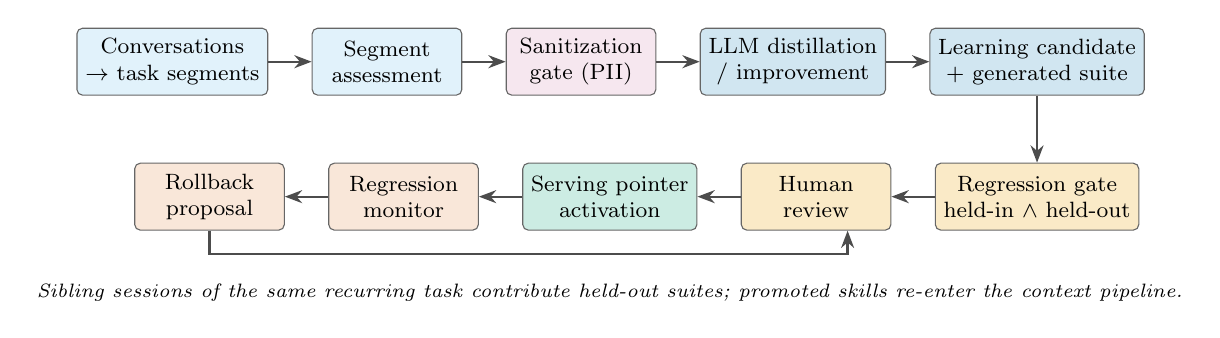
\begin{tikzpicture}[
  font=\footnotesize,
  node distance=0.55cm and 0.55cm,
  box/.style={rectangle, draw=black!60, rounded corners=2pt, minimum height=0.85cm,
              minimum width=1.9cm, align=center, inner sep=3pt},
  arrow/.style={-{Stealth[length=2.2mm]}, thick, black!70},
]
  \node[box, fill=okcyan!18] (seg) {Conversations\\$\to$ task segments};
  \node[box, fill=okcyan!18, right=of seg] (assess) {Segment\\assessment};
  \node[box, fill=okpurple!18, right=of assess] (sanitize) {Sanitization\\gate (PII)};
  \node[box, fill=okblue!18, right=of sanitize] (distill) {LLM distillation\\/ improvement};
  \node[box, fill=okblue!18, right=of distill] (cand) {Learning candidate\\+ generated suite};

  \node[box, fill=okorange!22, below=0.85cm of cand] (gate) {Regression gate\\held-in $\wedge$ held-out};
  \node[box, fill=okorange!22, left=of gate] (review) {Human\\review};
  \node[box, fill=okgreen!20, left=of review] (serve) {Serving pointer\\activation};
  \node[box, fill=okred!15, left=of serve] (monitor) {Regression\\monitor};
  \node[box, fill=okred!15, left=of monitor] (rollback) {Rollback\\proposal};

  \draw[arrow] (seg) -- (assess);
  \draw[arrow] (assess) -- (sanitize);
  \draw[arrow] (sanitize) -- (distill);
  \draw[arrow] (distill) -- (cand);
  \draw[arrow] (cand) -- (gate);
  \draw[arrow] (gate) -- (review);
  \draw[arrow] (review) -- (serve);
  \draw[arrow] (serve) -- (monitor);
  \draw[arrow] (monitor) -- (rollback);
  \draw[arrow] (rollback.south) -- ++(0,-0.3) -| ($(review.south)+(0.4,0)$);
  \node[align=center, anchor=north, font=\scriptsize\itshape] at ($(monitor.south)!0.5!(review.south)+(0,-0.55)$)
    {Sibling sessions of the same recurring task contribute held-out suites; promoted skills re-enter the context pipeline.};
\end{tikzpicture}%
}
\caption{The regression-gated skill learning loop. Successful task segments are assessed, sanitized, and distilled into candidate skills; each candidate must clear a paired non-regression gate over its own generated suite \emph{and} a held-out pool of sibling suites before human review moves the serving pointer. A monitor watches post-promotion resolution rates and files rollback proposals.}
\label{fig:pipeline}
\end{figure}

\section{Related work}
\label{sec:related}

\textbf{Skill libraries and experience learning.} A growing line of work has agents accumulate reusable procedural knowledge from their own trajectories: executable skill libraries verified by environment execution~\citep{wang2023voyager}, workflow induction from web navigation~\citep{wang2024awm}, distilled cross-task insights~\citep{zhao2023expel}, interactively learned environment manuals~\citep{chen2024automanual}, self-synthesized and practiced API skills~\citep{zheng2025skillweaver}, computer-control skills from screen interaction~\citep{tan2024cradle}, and continually updated causal memories~\citep{majumder2023clin}. \moa{} shares the distill-experience-into-artifacts premise (in the SKILL.md package format~\citep{anthropic2025skills, agentskills2026spec}) but differs on the admission side: in these systems validation is execution success in a sandboxed environment, LLM self-judgment, or downstream benchmark reward, and none interposes a governed release lifecycle (human review, typed provenance, monitored rollback, and a sanitization boundary that keeps raw transcripts out of the learning path) between distillation and serving.

\textbf{Contemporaneous regression-gated skill evolution.} In the months preceding this preprint, the admission side became an active direction of its own. GRASP treats skills as gated edits admitted only after a balanced held-out probe under a regression budget~\citep{moll2026grasp}; SkillOpt accepts a skill edit only when it strictly improves held-out validation performance~\citep{yang2026skillopt}; Self-Harness admits harness modifications via held-in plus held-out regression testing with a conservative no-degradation rule and repeated evaluation under stochasticity~\citep{zhang2026selfharness}; and the Regression Tax quantifies empirically that skills materially regress previously solved tasks~\citep{tank2026regressiontax}, which is the failure mode our comparator exists to catch. Ground-truth-free admission also has direct precedents: SkillAudit evolves skills without external ground truth via paired trajectory auditing against a fixed structural verifier~\citep{gao2026skillaudit}, and Self-Supervised Skill Optimization gates updates on an unlabeled validation set using comparative LLM judgments~\citep{peng2026sso}. Held-out gating of self-modification is therefore no longer novel in itself. Our focus is complementary and one layer down: these systems presuppose an evaluation signal (benchmark outcomes, verifier scores, or judge preferences), whereas we construct the \emph{test oracle itself} from ordinary unlabeled traffic, by deterministically corroborating typed response spans against successful tool-result evidence and persisting them as regression assertions inside a governed release lifecycle. ProvenanceGuard's observation that pooled evidence can support a claim while misattributing which source supports it~\citep{alvarez2026provenanceguard} sharpens a limitation our concatenated grounding corpus shares (\S\ref{sec:limitations}).

\textbf{Self-improvement and its safety.} Self-refinement and self-training methods~\citep{madaan2023selfrefine, shinn2023reflexion, zelikman2022star} and, at the extreme, self-modifying agent populations gated by benchmark scores~\citep{zhang2025dgm} form a fast-moving space with dedicated surveys~\citep{tao2024selfevolution, gao2025selfevolving}. The accompanying safety literature documents model collapse from self-generated data~\citep{shumailov2023curse} and reward hacking of proxy objectives~\citep{pan2022rewardmisspec}. \moa{} takes these as design constraints: improvement is confined to auditable declarative documents (never weights, never raw trajectories), the gate signal is exact corroboration rather than a learned or judged score, generalization is measured on held-out sibling sessions, and every promotion is reversible.

\textbf{Verifying agent outputs without labels.} Existing label-free verification uses LLM judges, whose biases are well documented~\citep{zheng2023llmjudge, wang2023fairevaluators}; agreement- and execution-based proxies~\citep{wang2022selfconsistency, chen2022codet}; or evidence-grounding checks developed for attribution: the AIS framework~\citep{rashkin2023ais}, attributed QA~\citep{bohnet2022attributedqa}, citation evaluation~\citep{gao2023alce}, post-hoc revision~\citep{gao2023rarr}, sampling-based hallucination detection~\citep{manakul2023selfcheckgpt}, and atomic-fact factual-precision scoring~\citep{min2023factscore}. The grounded-facts oracle belongs to the evidence-grounding family but repurposes it: rather than scoring attribution quality of free text against retrieved documents with NLI models or judges, it extracts high-precision typed spans and requires exact word-boundary corroboration in the session's own tool outputs, yielding a deterministic pass/fail oracle used not to score single responses but to \emph{generate regression suites} that gate promotion.

\textbf{Behavioral testing and safe deployment.} CheckList brought suite-based behavioral testing to NLP models~\citep{ribeiro2020checklist}, and the ML Test Score codified testing and monitoring for production pipelines~\citep{breck2017mltestscore}; a parallel thread studies regressions from model updates: negative flips~\citep{yan2021pctraining}, update regression~\citep{cai2022updateregression}, and behavioral drift of deployed LLM APIs~\citep{chen2023chatgptbehavior}. Deriving test oracles from observed executions has a long software-engineering lineage~\citep{pacheco2007randoop}, and benchmarks for tool-agent interaction increasingly stress verifiable end states~\citep{yao2024taubench}. The MLOps literature motivates staged rollout, monitoring, and rollback~\citep{sculley2015hidden, paleyes2022challenges, shankar2022operationalizing, amershi2019se4ml}. \moa{} transplants this discipline to in-context skill artifacts: generated suites are pre-deployment tests derived from real traffic rather than hand-written templates, sibling suites act as shadow evaluation, the resolution-rate monitor is the canary metric, and rollback proposals close the loop. Concerns about benchmark overfitting and contamination~\citep{sainz2023contamination, li2023taskcontamination, kapoor2024aiagents} appear here as an internal threat, partially addressed architecturally (\S\ref{sec:gate}).

\section{System overview}
\label{sec:system}

\moa{} is a multi-tenant enterprise agent platform written in Rust, with durable orchestration on Restate and tenant state in Postgres. Four properties of the surrounding platform matter for this paper. First, every conversation is an append-only event log; tool calls, tool results, approvals, and responses are typed events that can be replayed. Second, work is measured in \emph{task segments}: contiguous spans of a session bounded by task-boundary signals, each closed by a deterministic \emph{segment assessment} that scores resolution from five weighted signal classes (tool outcomes, verification events, user continuation behavior, model self-assessment, structural features) into an outcome in $\{$\code{Resolved}, \code{Partial}, \code{Unknown}, \code{Failed}, \code{Abandoned}$\}$ with a confidence score. Third, all learning state is tenant-scoped: skills, candidates, and logs never cross tenant boundaries. Fourth, every learned behavior is required to have provenance and a rollback path, a platform design value that predates and motivates the mechanism described here.

Resolved segments become \emph{experience records}: task fingerprint, facets, tools used, outcome, confidence, and typed attributions of which skills, tools, or memories helped or harmed. Experiences are the sole input to skill learning. The complete loop (Figure~\ref{fig:pipeline}) is: experiences are sanitized and distilled into candidate skills; candidates are filed with a deterministically generated regression suite; the review-time gate executes that suite and a held-out sibling pool; a human reviewer accepts or rejects; acceptance transactionally activates a new skill revision behind a serving pointer; a monitor watches post-promotion resolution rates and files rollback proposals. Skills are Agent-Skills-style packages (YAML frontmatter plus a Markdown procedure body, optional scripts and references, and the generated suite at \code{tests/regression-suite.toml}), injected into future context by relevance ranking with progressive disclosure of body and resources.

\section{Regression-gated skill learning}
\label{sec:method}

\subsection{Admission: which experiences may teach}
\label{sec:admission}

Not every success is worth learning from, and not every learnable success is releasable. A \emph{learnability gate} requires \code{Resolved} outcomes to carry confidence $\geq 0.7$; \code{Partial} outcomes need confidence $\geq 0.85$ \emph{and} a helpful attribution \emph{and} corroborating verification evidence; failed or abandoned segments never teach. A tool-call floor (default 8; relaxed to 3 for recurring tasks) filters out trivial segments whose ``procedure'' is a single lookup. One assumption should be explicit: \code{Resolved} is not ground truth. It is the output of the deterministic composite assessment (\S\ref{sec:system}), whose signals include model self-assessment. When we say the pipeline needs no labels, the precise claim is that \emph{no human task labels, reference answers, or external reward are required to construct the promotion assertions}; the admission layer produces heuristic outcome labels, and this paper conditions on that layer identifying learnable experience correctly rather than validating it.

Before any model call, a \emph{sanitization gate} converts the segment's events into a sanitized evidence value, \code{SanitizedLearningEvidence}. Every carrier passes a PII classifier: user messages, assistant responses and reasoning summaries, tool arguments (walked as JSON, key and value position), tool results and errors, memory paths, task summaries. Redactions are re-classified for residual sensitivity, and any refusal (restricted class, credential material, classifier abstention) ends the learning pass with zero writes and zero provider calls. The type has no raw-string constructor and no deserializer, so code paths downstream of the gate cannot bypass the sanitizer API to represent unsanitized text. That is a guarantee about the type boundary, not about the classifier: a false negative still passes whatever the classifier missed. This is the structural answer to a compliance question every self-learning production system faces (what if the model memorializes a customer's data into a reusable artifact?), and it also constrains the oracle design in \S\ref{sec:oracle}: expectations must survive redaction.

Distillation is a single auxiliary-model call that turns sanitized evidence into a complete SKILL.md (when-to-use guidance, numbered procedure, pitfalls, verification steps), explicitly instructed to learn durable workflow structure and not to copy transient identifiers. Routing between \emph{creating} a new skill and \emph{improving} an existing one is decided by embedding similarity against serving skills (cosine threshold 0.80, with a lexical Jaccard fallback); near-duplicate proposals are deduplicated onto open candidates, whose suites accumulate as siblings (\S\ref{sec:gate}). A deterministic \emph{recurrence miner} clusters exact and near-duplicate task fingerprints (embedding union-find, similarity 0.85) and, when a loop recurs $\geq 3$ times in 30 days, distills the best exemplar while feeding the remaining members through the same sanitization gate as held-out material. A complementary \emph{weakness miner} clusters recurring failure signals into non-reviewable authoring candidates; mining observes that something keeps failing, but does not produce a change anything can auto-apply.

\subsection{The grounded-facts oracle}
\label{sec:oracle}

At proposal time---deterministically, with no model call---\moa{} generates a regression suite from the source segment. The suite's test case replays the segment's opening user message as input; its blocking assertions are (i) \emph{response-carries-source-facts}: the candidate's response must contain the expected output set, and (ii) \emph{recorded-tools-were-used}: the candidate must use the distinct set of tools the successful run used. A third assertion records the observed tool \emph{order} but is diagnostic-only (\S\ref{sec:lessons}).

The expected output set is where the verification signal lives. The generator scans the final assistant response, in order of first appearance, for five classes of typed spans: quoted or backticked text (3--80 bytes); URLs; file paths; numbers with optional grouping, currency prefixes, and unit suffixes (\code{45ms}, \code{\$1,200}, \code{12\%}), excluding trivial bare integers 0--2 and bare years; and identifiers (UUIDs, reference tokens like \code{ABC-123}, commit hashes, \code{snake\_case}/\code{camelCase} names). Each candidate fact is tested against a \emph{grounding corpus}: the concatenated text of the session's \emph{successful, non-error} tool results only. Denied calls, failed executions, and tool errors are excluded, so failure identifiers can never become required expectations. A fact grounds if it occurs in the corpus case-insensitively with word boundaries on both sides (a word character being ASCII alphanumeric or underscore): \code{42} does not ground against \code{1420}, and \code{45ms} does not ground against \code{845ms}, but punctuation-edged facts like \code{\#482} and \code{\$1,200} match exactly. The boundary check protects against alphanumeric extensions only; because \code{.}, \code{-}, and \code{/} are non-word characters, a fact can still ground against a punctuation-extended variant (\code{\$1,200} against \code{\$1,200.99}), a precision gap we measure in \S\ref{sec:casestudy} and whose fix (typed per-class canonicalization) we outline there. The first five grounded facts (deduplicated, $\leq$80 bytes each) become the expected output; the suite records its oracle kind as \code{GroundedFacts}. If nothing grounds (no tool results, or a response whose spans none trace to a tool), the generator falls back to a \code{Keywords} oracle over a fixed subset of the response's longer tokens (length $\geq 5$, lowercased, deduplicated) and records that, so reviewers and reports can distinguish fact-grounded cases from fallback cases.

What does a pass certify? \code{GroundedFacts} verifies \emph{preservation of selected tool-supported literals}: a passing candidate demonstrably carried spans forward that some successful tool result also produced. It is a necessary evidence-faithfulness signal, not a sufficient verifier of semantic correctness or task completion. It does not establish that the tool result was itself correct, that the fact was relevant to the question, that the response interpreted it correctly, that no contradictory tool result existed, or that the task was completed. Corroboration across carriers (response \emph{and} tool output, produced by different mechanisms) is what makes even this weaker signal hard to satisfy vacuously; the surrounding lifecycle (tool-set assertion, held-out siblings, human review, rollback monitor) is what the design relies on for the rest. The oracle is deterministic and auditable: a reviewer reading the suite TOML sees exactly which facts the gate will demand and where they came from.

\subsection{The two-sided gate: held-in and held-out}
\label{sec:gate}

A suite generated from session $s$ cannot, alone, certify a skill distilled from session $s$; that would grade a draft on the cases it was derived from and report a passing held-out split that held nothing out. \moa{} therefore accumulates \emph{sibling suites}: when another session of the same recurring task deduplicates onto an open candidate, or a recurrence cluster distills its exemplar, suites generated from those \emph{other} sessions (each independently sanitized) attach to the candidate as held-out contributions, up to a cap of three. Storage enforces the split: the candidate's own suite is recorded as \code{Generated}; only \code{Accumulated} sibling rows feed the held-out pool. For an improvement to an existing skill, the pool additionally contains the previous promoted revision's own suite, so the new revision is tested on the material that admitted its predecessor. Two scoping notes. First, this construction \emph{structurally prevents direct same-session test leakage}; it does not prevent all adaptive overfitting. Sibling sessions may be highly similar, predecessor suites are reused across revisions, and a proposer that inspects a held-out failure before revising has partially exposed that test. Second, sibling validity rests on the recurrence-identity mechanism (embedding clustering at fixed thresholds, \S\ref{sec:admission}): a false merge attaches an unrelated session's suite as bogus held-out material, and a false split forfeits held-out coverage. We do not evaluate clustering accuracy in this paper; the study conditions on it.

At review time, the gate compiles both packages---previous serving revision and candidate---into eval agents that differ \emph{only} in the injected skill markdown (otherwise the score comparison is vacuous), and runs the suites under a fixed evaluator set with a hard cost ceiling (default \$0.50 per gate). A candidate whose estimated evaluation cost exceeds the budget is currently rejected outright; this makes gate cost a bounded design parameter, but conflates ``candidate is bad'' with ``we declined to spend enough to evaluate it,'' and a distinct deferred-evaluation state would be the cleaner design.

Where do tool results come from at review time? Eval agents run against a live model provider with the platform's real tool router over an \emph{isolated temporary sandbox workspace}: never live tenant systems, and no replay of recorded tool outputs. Facts the sandbox can reproduce (file contents, computed values, tool-mediated state the skill itself establishes) discriminate between revisions; environment-dependent facts that cannot reproduce fail both runs equally, and the comparator below neutralizes them. We call the candidate's own suite the \emph{held-in} side of the gate and the sibling/predecessor pool the \emph{held-out} side. Scoring averages blocking assertions only.

The acceptance criterion is not ``the candidate passes its tests'' but a \emph{paired non-regression comparison against the serving revision}: fewer failed runs wins outright; equal failures require average score $\geq$ baseline. The epsilon in that comparison guards floating-point representation, not model sampling variance; the eval-agent runs themselves are stochastic, and repeated paired trials, as Self-Harness runs under its no-degradation rule~\citep{zhang2026selfharness}, would be the statistically principled upgrade. A first revision with no predecessor instead faces an \emph{absolute} criterion (candidate-only execution with zero failures), which exposes an asymmetry: for improvements, an environment-dependent fact that cannot reproduce in the sandbox fails both runs and neutralizes, but a first revision has no paired run to neutralize against, so a valid skill distilled from an environment-dependent result may be structurally unable to clear its smoke gate. Record/replay fixtures for read-only tools, or an explicit non-reproducible state, would close this gap. Two further asymmetries are deliberate. Operational failures (provider outage) do not waive the gate; they release the review claim so the review can be retried, and are recorded separately from candidate failures. And the held-out comparison tolerates environmental staleness: a pooled case that errors identically under both revisions neutralizes itself; only the candidate doing \emph{worse} than its predecessor on material it never saw is a regression.

Finally, the keyword fallback. Our own measurements (\S\ref{sec:casestudy}) show it behaves as near-verbatim matching, rejecting every innocuous rewording. A design more consistent with the platform's fail-closed philosophy would have the automatic gate \emph{abstain} when no sufficiently strong grounded evidence exists, routing such candidates to human or domain-specific verification instead of certifying them against keywords. We consider that the right next change to the system.

\subsection{Promotion, provenance, rollback}
\label{sec:lifecycle}

Candidates move \code{Proposed} $\to$ \code{Evaluating} $\to$ \code{Promoted}~$|$~\code{Rejected}; both accept and reject first claim the candidate, bound to a request digest, so concurrent reviewers cannot both succeed and retries replay rather than re-execute. Acceptance requires \code{AcceptanceChecks} derived from what actually executed (including whether any held-out material existed) and activates the new revision inside one transaction through the platform's shared release contract: validation report, release-candidate record with the gate report's hash as the plan hash, decision record with per-gate results, and a compare-and-set move of the tenant's \emph{serving pointer}. There is no \code{published} status on skill artifacts; visibility is owned by the pointer, which makes activation atomic and rollback a pointer operation rather than a data migration. Every promotion appends \code{skill\_created} or \code{skill\_improved} to an append-only, bitemporal learning log with typed source provenance; rollback invalidates by setting \code{valid\_to}, never by deletion.

After promotion, a deterministic monitor (no model calls) compares the skill's segment resolution rate in a 14-day window after activation against the pre-promotion baseline. It abstains below five samples; for improvements it files a rollback proposal when the post rate drops more than $0.2$ below baseline, and for newly created skills (no baseline) when the post rate falls below an absolute floor of $0.3$. This monitor should be read as an \emph{operational heuristic}, not a statistically supported regression detector: five samples is very noisy for a rate metric, and naive before/after comparison is confounded by task mix, model and tool changes, and traffic shifts. A stronger version would condition on the same task family with the skill actually activated and attach interval estimates; recent measurements that skills materially regress previously solved tasks~\citep{tank2026regressiontax} motivate investing there. Rollback proposals are themselves reviewable candidates carrying the full evidence (rates, sample counts, revision and audit identifiers), keyed to the exact serving epoch so a re-activation cannot inherit stale evidence. Accepting one archives the regressed revision and tombstones its pointer, leaving the skill \emph{unserved} rather than silently restoring a predecessor, which would bypass the gate. This is a deliberate availability-for-safety trade: after a rollback of an improvement, no revision serves until a replacement clears its own gate, rather than reverting to a predecessor whose gate evidence may no longer be valid for the current environment.

\section{Case study: does the oracle measure what it claims?}
\label{sec:casestudy}

Live promotion metrics require production traffic and are deferred to future work (\S\ref{sec:limitations}). What we can establish now, rigorously, is whether the oracle has the discrimination properties the design claims: that it accepts faithful and semantically equivalent reruns, rejects fabricated or evidence-free results, refuses spurious grounding, and tolerates legitimate procedural variation. Because suite generation and assertion evaluation are deterministic, these properties are measurable exactly on the constructed test distribution; determinism removes run-to-run measurement noise, though not the construction uncertainty of generalizing beyond these cases (\S\ref{sec:limitations}). The harness drives the production code paths: the real sanitization gate (\code{sanitize\_segment\_evidence} with the production PII classifier), the real generator (\code{generate\_skill\_test\_suite\_source}), and the real gate-time evaluators (\code{evaluate\_assertions} over the built-in registry), fed synthetic task segments with planted, typed facts. It is seeded, makes no network or model calls, and is released with the paper. Segments embed facts of eight types in tool results, with final responses carrying a controlled number of those facts verbatim; the characterization experiment sweeps $t \in [2,8]$ tool calls and $k \in [0,5]$ carried facts.

\textbf{Oracle selection and determinism (n=300).} The generator chose the \code{GroundedFacts} oracle in exactly the 250 segments whose response carried at least one tool-corroborated fact and fell back to \code{Keywords} in exactly the 50 segments with none ($k{=}0$); repeated generation produced identical assertion sets and oracle choices in 300/300 cases. Grounded cases asserted a median of 4 facts (cap 5), dominated by numeric and currency spans (including incidental grounded spans beyond the planted facts), with UUIDs and reference tokens where planted.

\textbf{Adversarial grounding, alphanumeric (n=200).} With tool outputs corrupted so that every response fact appears only as a strict substring of a longer alphanumeric token (\code{412ms} inside \code{1412msx}), the word-boundary check refused to ground in 200/200 segments: zero false groundings on this adversarial family.

\textbf{Adversarial grounding, punctuation extensions (n=300).} The boundary rule does not protect against extensions that begin with a non-word character; we owe this measurement to adversarial review of an earlier draft. Across six families---currency (\code{\$1,200} vs.\ tool output \code{\$1,200.99}), reference tokens (\code{ABC-123} vs.\ \code{ABC-123-456}), paths (\code{/tmp/foo} vs.\ \code{/tmp/foo/bar}), URL prefixes, decimals (\code{12} vs.\ \code{12.5}), and hyphenated units (\code{412ms} vs.\ \code{412ms-related})---the response fact falsely grounded against the punctuation-extended tool token in \textbf{300/300 cases}. The precision boundary is the word-character definition itself: safe against alphanumeric extension, systematically unsafe against punctuation extension. The fix is typed per-class canonicalization (parse and compare complete monetary tokens, normalized URLs, full path segments, and value-unit pairs, rather than applying one universal boundary regex) plus per-fact provenance recording the originating tool call and byte span, which would also address the source-conflation risk that pooled grounding corpora share~\citep{alvarez2026provenanceguard}.

\begin{table}[t]
\centering
\caption{Gate outcomes under response perturbations, grounded-facts oracle versus its own keyword fallback (200 segments each; deterministic, so rates are exact). Fabrication and omission rows are spec-conformance checks (string-level mutations of planted facts); the paraphrase row is the empirical contrast: keywords reject every fact-preserving paraphrase, behaving as brittle near-verbatim matching.}
\label{tab:perturbation}
\small
\begin{tabular}{llcc}
\toprule
Candidate response & Desired verdict & Grounded facts & Keyword fallback \\
\midrule
Exact reproduction & pass & \textbf{100\% pass} & 100\% pass \\
Planted-fact-preserving paraphrase & pass & \textbf{92.5\% pass} & 0\% pass \\
Facts fabricated (digits mutated) & fail & \textbf{100\% fail} & 100\% fail \\
Facts omitted (fluent, evidence-free) & fail & \textbf{100\% fail} & 100\% fail \\
\bottomrule
\end{tabular}
\end{table}

\textbf{Perturbation detection (n=200 segments $\times$ 4 variants $\times$ 2 oracles).} Table~\ref{tab:perturbation} summarizes the central result. Two kinds of rows must be distinguished. The fabrication and omission rows (and the alphanumeric adversarial check above) are \emph{spec-conformance} results: the perturbations are string-level mutations of planted facts, so a correct implementation of exact matching is expected to detect them at 100\%, and the value of the measurement is confirming the deployed implementation meets its spec with no false groundings. The \emph{empirical} finding is the selectivity contrast between the two oracles on paraphrases. Under the grounded-facts oracle, exact reruns always pass; responses whose facts were fabricated (every digit mutated, preserving format) or omitted (fluent text, no evidence) always fail the blocking fact assertion. Planted-fact-preserving paraphrases pass 92.5\% of the time on this finite deterministic suite; inspection shows all 15 false rejections trace to a single cause. The oracle had additionally grounded an incidental enumeration digit (``Finding 3'' matching a step index in tool output, since the trivial-number floor excludes only 0--2 and years), and the paraphrase dropped it. The keyword fallback detects fabrication identically but rejects \emph{every} paraphrase: asserting a fixed set of the response's longer tokens makes it a near-verbatim match on arbitrary wording. The grounded oracle's advantage is not detection but \emph{selectivity}: it pins the spans that carry the task's result and frees everything else to vary. This is the measured justification for preferring grounded facts wherever they exist, and the case against letting keywords participate in automatic certification at all (\S\ref{sec:gate}).

\textbf{Action assertions (n=200).} The distinct-tool-set assertion detected a dropped tool in 200/200 runs, while a maximally rerouted trajectory (reversed order with a duplicated call, \emph{same distinct set}) passed 200/200. Scope matters here: what is tolerated is alternative \emph{orderings and repetition} over the recorded tool set, not alternative routes. A candidate that reaches the same verified result through a different tool set, including a genuine improvement that eliminates an unnecessary call, fails the assertion by design. This is a deliberate conservatism (the dropped-tool row is that same behavior, viewed as detection); the natural relaxation is capability-level requirements derived from each fact's originating tool.

\section{Design lessons}
\label{sec:lessons}

\textbf{A trajectory-similarity gate was built, then deleted.} An earlier revision gated candidates on longest-common-subsequence similarity between the candidate's tool trajectory and the recorded one. It punished exactly the wrong thing: a candidate that reached the same verified result by a shorter or reordered route failed, while the assertion said nothing about whether the \emph{result} was real. The replacement demands the distinct tool set (was the capability used at all?) as blocking, and reports order as a diagnostic---one observation of one run, not a requirement. The case study's reroute result (\S\ref{sec:casestudy}) measures the replacement's tolerance directly.

\textbf{Fail closed, everywhere.} Suites declare a schema version, and older versions are rejected outright rather than partially parsed: a silently ignored expectation block would turn into a vacuous pass. Assertions name registry evaluators with versions; an unknown evaluator fails the case rather than skipping it. An empty evaluator configuration still runs assertions, so a suite cannot dodge its claims. The same posture governs sanitization (refusal ends the pass with zero writes) and the monitor (abstains below minimum samples rather than guessing).

\textbf{Keep quality signals out of the artifact.} Use counts, success rates, and rollback history live in revisions, candidates, and the learning log, never in SKILL.md, whose unsupported metadata keys are rejected at parse. The artifact a reviewer reads is exactly the artifact the agent executes; runtime state cannot smuggle itself into a promoted document.

\textbf{Determinism is a reviewability feature, with limits.} Because suite generation and assertion evaluation are deterministic, a reviewer sees the exact facts the gate will demand, an auditor can regenerate the suite from the sanitized evidence and obtain the same assertions, and the platform can replay a promotion decision from its request digest. The gate \emph{verdict} is not fully deterministic: it rests on stochastic eval-agent runs against a live provider. What determinism buys is that every nondeterministic contribution is confined to those runs, and everything that specifies, scores, and records them is reproducible. Within the gate itself, the model appears in two places (writing the skill document and executing the eval runs), and neither can alter what the gate demands. The wider pipeline does use models elsewhere, in routing embeddings and in a self-assessment component among the segment-assessment signals, which is why we scope the claim to the gate.

\section{Threat model}
\label{sec:threats}

A multi-tenant system that learns durable artifacts from its own traffic must consider adversaries, and PII sanitization is not poisoning protection. We enumerate the threats the design faces and its current posture on each. \emph{Poisoned evidence}: an attacker can place reusable malicious instructions in user text, tool outputs, ticket bodies, or fetched web content, hoping distillation memorializes them into a served skill. The platform routes tool traffic through a security layer with prompt-injection controls and outbound-destination policy, and the distillation prompt instructs the model to learn workflow structure rather than copy content. But the learning path's primary defenses are the gate (injected instructions do not help a candidate reproduce grounded facts), human review of every promotion, and rollback; none of these is proof against a skill that is both malicious and task-effective. \emph{Compromised or wrong tools}: the oracle trusts successful tool results as its grounding corpus, so a tool that returns attacker-controlled or incorrect data grounds incorrect facts; provenance-aware per-tool grounding (\S\ref{sec:casestudy}) would narrow but not remove this. \emph{Sanitizer false negatives}: the type boundary prevents bypassing the sanitizer, not classifier misses (\S\ref{sec:admission}). \emph{Recurrence flooding}: an attacker who can generate many similar sessions can manufacture a recurring task and its sibling suites; tenant isolation confines the blast radius to the attacker's own tenant, and per-tenant candidate caps bound the volume, but within a tenant this remains a review-burden attack. \emph{Held-out leakage}: a proposer that observes held-out failures across repeated proposals gradually exposes the pool (\S\ref{sec:gate}); rotating holdout material across generations would mitigate this. \emph{Privilege escalation via skill text}: a skill's prose could instruct the agent toward tools beyond its remit, but runtime tool policy is compiled at the agent and turn level and enforced at dispatch; it is not read from skill text, so prose alone cannot widen permissions. The frontmatter \code{allowed-tools} declaration does influence the agent's resolved tool set, and it enters that set only as part of the reviewed, gated artifact. We present this enumeration as a design map, not a security evaluation; adversarial testing of the learning path is future work.

\section{Limitations}
\label{sec:limitations}

The case study characterizes the oracle's discrimination properties on synthetic segments constructed to be groundable (the planted facts match the extractor's span classes by design), so its detection rows verify the implementation rather than estimate real-world recall, and the paraphrase variants keep fact spans byte-identical, making 92.5\% an upper bound on a favorable distribution. The oracle demands surface-form-exact reproduction: a rerun that reformats a fact (\code{412ms} vs.\ \code{0.41s}, \code{\$1,200} vs.\ \code{1200 USD}) is rejected, and quantifying that cost on harder, model-generated paraphrases is needed before the selectivity number can be taken at face value. False rejections also compound across a gate's cases: at the observed 7.5\% per-case rate, a candidate facing four independent cases would be falsely rejected roughly a quarter of the time, a reviewer-burden cost the design pays for conservatism. The study also does not compare against an LLM-judge baseline on the same perturbation grid, which would quantify what the deterministic oracle gives up; nor does it measure end-to-end improvement of a deployed fleet. The decisive production questions (what fraction of promoted skills raise resolution rates, how often the monitor fires, what the reviewer burden is) require live tenant traffic and are the subject of ongoing measurement; this paper documents the mechanism and its verifiable properties, and we intend a follow-up with longitudinal deployment data. The oracle's precision has two measured soft edges: incidental grounded spans (enumeration digits, step indices) can over-constrain paraphrased reruns, and punctuation-extended tool tokens falsely ground response facts at 100\% in the tested families (\S\ref{sec:casestudy}); ranked typed fact selection with per-class canonicalization and per-fact provenance addresses both and is the highest-priority implementation refinement. The false-rejection compounding estimate above also assumes case independence, which correlated incidental spans violate. The oracle also inherits the limits of its corpus: tasks whose success leaves no verbatim trace in tool outputs (pure advice, summarization) fall back to keywords, and a response could in principle echo tool output without correctly completing the task; the tool-set assertion and human review bound but do not eliminate this. Held-out siblings measure generalization across sessions of the \emph{same} recurring task, not transfer to novel tasks. Finally, single-case suites per session keep gate cost inside a \$0.50 budget but bound per-candidate statistical power; the design compensates with accumulation over time rather than breadth per gate.

\section{Conclusion}
\label{sec:conclusion}

Self-improvement in production is a release-engineering problem before it is a learning problem. With held-out gating of self-modification now an active research direction~\citep{moll2026grasp, yang2026skillopt, zhang2026selfharness}, the contribution we defend sits one layer beneath the gate: deterministic regression assertions constructed from tool-corroborated facts in unlabeled traces, wrapped in a lifecycle that treats each learned skill as a governed artifact. A skill is admitted only from sanitized, high-confidence experience; cleared by paired non-regression against the serving revision, on material including held-out sibling sessions; promoted atomically behind a serving pointer by a human decision with full provenance; and watched by a monitor that can propose its removal. Within its string-level perturbation model, the case study shows the oracle detects every fabricated or evidence-free result and accepts nearly all planted-fact-preserving paraphrases, a selectivity the keyword baseline lacks entirely; the punctuation-extension study locates the matcher's real precision boundary and fixes its direction of improvement. Concrete next steps: typed canonicalization and per-fact provenance in the matcher; abstention in place of the keyword fallback; longitudinal measurement of promotion outcomes on live tenant traffic; and extending sibling pooling across tenants under differential-privacy constraints, so that recurring tasks common to many organizations can be learned once, gated everywhere.

\bibliographystyle{plainnat}
\bibliography{references}

\appendix

\section{Gate and oracle constants}
\label{app:constants}

Table~\ref{tab:constants} lists the default configuration governing the mechanism, as shipped. All are tenant-configurable except structural invariants (schema versioning, the held-out exclusion of \code{Generated} suites, and the sanitization gate, which cannot be disabled).

\begin{table}[h]
\centering
\caption{Default constants of the learning loop.}
\label{tab:constants}
\footnotesize
\setlength{\tabcolsep}{4pt}
\begin{tabular}{lll}
\toprule
Component & Constant & Default \\
\midrule
Learnability & \code{Resolved} confidence floor & 0.70 \\
 & \code{Partial} floor (needs attribution + verification) & 0.85 \\
 & minimum tool calls (single-session / recurrence) & 8 / 3 \\
Routing & improve-vs-create cosine similarity & 0.80 \\
 & proposal dedupe similarity & 0.85 \\
Recurrence & occurrences / lookback / cooldown & 3 / 30 d / 30 d \\
 & cluster similarity & 0.85 \\
Oracle & max facts per case / max fact length & 5 / 80 bytes \\
 & trivial numbers excluded & 0--2, years 1900--2099 \\
Gate & budget per gate / suite timeout floor & \$0.50 / 90 s \\
 & held-out sibling cap & 3 \\
 & pass criterion & fewer failures, else score $\geq$ baseline \\
Monitor & min samples / lookback & 5 / 14 d \\
 & regression delta (improved) / floor (created) & 0.2 / 0.3 \\
\bottomrule
\end{tabular}
\end{table}

\section{Reproducing the case study}
\label{app:repro}

The harness is a single-file Rust crate that path-depends on the platform's crates and ships the workspace lockfile; \code{cargo run} regenerates every number in \S\ref{sec:casestudy} deterministically (seeds 7, 11, 23, 31, 47; no network, no model calls, $\sim$1 minute on a laptop). Segments are synthesized as typed event logs (user message, tool call/result pairs, final response) and pass through the production sanitization, generation, and evaluation entry points; perturbations mutate only the candidate response text or action ledger presented to the evaluators. Paraphrase variants are template-generated: surrounding prose is rewritten while fact spans are preserved byte-identically (\S\ref{sec:limitations} discusses why this is the favorable case). Per-experiment counts: characterization 300 segments, alphanumeric adversarial grounding 200, punctuation-extension adversarial grounding 300, perturbation study 200 grounded + 200 keyword-twin segments, action assertions 200 (total 1{,}400); gate evaluations $200 \times 4 \times 2 + 200 \times 2 = 2{,}000$ (the adversarial studies exercise suite generation only). Code and the emitted \code{results.json} accompany the paper.

\end{document}
